% Course report (AMS style). Compile from this directory:
%   pdflatex report.tex && pdflatex report.tex
% Figures: run ``python ../scripts/make_paper_figures.py --demo --out_dir figures``
% after training, omit ``--demo`` and pass real CSV/JSON paths (see README).

\documentclass[10pt, reqno, letterpaper, twoside]{amsart}
\usepackage[margin=1in]{geometry}

\usepackage{amssymb, bm, mathtools}
\usepackage[usenames,dvipsnames,svgnames,table]{xcolor}
\usepackage[pdftex, xetex]{graphicx}
\usepackage{enumerate, setspace}
\usepackage{float, colortbl, tabularx, longtable, multirow, subcaption, environ, wrapfig, textcomp, booktabs}
\usepackage{pgf, tikz, framed, url, hyperref}
\usepackage[normalem]{ulem}
\usetikzlibrary{arrows,positioning,automata,shadows,fit,shapes}
\usepackage[english]{babel}

\usepackage{microtype}
\microtypecontext{spacing=nonfrench}

\usepackage{times}
\graphicspath{{figures/}}

\title{Lightweight Gaze Estimation for Real-Time Mobile Deployment via Knowledge Distillation}
\author{Your Name [yourname@seas.upenn.edu]}

\begin{document}

\begin{abstract}
We study two-dimensional gaze regression from face images with a compact model suitable for mobile deployment. A ResNet-18 teacher is trained with mean squared error (MSE) on image-to-gaze supervision, then a MobileNetV3-Small student is trained either with labels alone or with an additional MSE distillation term to the teacher's outputs. We compare accuracy, parameter count, checkpoint size, and single-image latency on the same validation split. On a synthetic ellipse--pupil dataset used for reproducible pipeline validation, distillation reduces the student's validation error relative to the baseline while preserving the student's efficiency advantage over the teacher. We discuss adapting the same codebase to MPIIGaze-style benchmarks and standard angular gaze metrics.
\end{abstract}

\maketitle

\section{Introduction}

Gaze estimation supports attention-aware interfaces, accessibility tools, and driver monitoring. Deep models can achieve strong accuracy but often rely on heavy backbones that are costly on phones or embedded GPUs. This project asks whether \emph{knowledge distillation} (KD) can improve a lightweight student network for 2D gaze regression without changing the inference architecture.

We keep the setup deliberately simple: inputs are RGB face crops; outputs are two continuous coordinates $(g_x, g_y)$. Training uses MSE against ground truth; the KD variant adds an MSE term between student and teacher predictions. The objective is not to match state-of-the-art angular error on in-the-wild data in a first pass, but to provide a clean, reproducible pipeline and an interpretable comparison between teacher, student baseline, and distilled student.

\subsection{Contributions}

\begin{itemize}
  \item A modular PyTorch codebase with CSV-based labels, ResNet-18 teacher, MobileNetV3-Small student, and KD training with configurable $\alpha$.
  \item Scripts to generate a synthetic dataset for quick experiments, log training curves, export evaluation JSON, and build PDF figures for the report.
  \item An empirical comparison of regression error, model size, and inference latency, with discussion of extending metrics and data to MPIIGaze.
\end{itemize}

\section{Background}

Let $\mathbf{I} \in \mathbb{R}^{3\times H \times W}$ denote a face image and $\mathbf{g} = (g_x, g_y)$ the target gaze vector. A network $f_\theta$ predicts $\hat{\mathbf{g}} = f_\theta(\mathbf{I})$. Supervised training minimizes
\[
  \mathcal{L}_{\mathrm{gt}}(\theta) = \big\lVert \hat{\mathbf{g}} - \mathbf{g} \big\rVert_2^2 .
\]
Given a fixed teacher $f_{\theta_T}$, distillation adds
\[
  \mathcal{L}_{\mathrm{kd}}(\theta_S) = \big\lVert f_{\theta_S}(\mathbf{I}) - f_{\theta_T}(\mathbf{I}) \big\rVert_2^2 ,
\]
and we minimize $\mathcal{L}_{\mathrm{gt}}(\theta_S) + \alpha \mathcal{L}_{\mathrm{kd}}(\theta_S)$ with the teacher in eval mode and gradients disabled. This matches regression KD with MSE targets; more advanced variants match intermediate features or temperature-scaled logits in classification.

\section{Related Work}

Appearance-based gaze estimation was popularized in part by MPIIGaze~\cite{zhang15mpiigaze}, which records everyday laptop users and provides normalized eye images and calibration-aware labels. Many follow-ups explore larger architectures, multi-task learning, and geometry-aware losses. For mobile deployment, efficient CNNs such as MobileNetV3~\cite{howard19mobilenetv3} trade accuracy for fewer multiply-adds. Knowledge distillation~\cite{hinton15kd} transfers information from a large teacher to a smaller student; we use the simplest output-level MSE form for transparency in a course setting.

\section{Approach}

\paragraph{Data interface.} Images and labels are listed in CSV files with columns \texttt{image\_path}, \texttt{gaze\_x}, \texttt{gaze\_y}. Paths may be absolute or relative to a configurable root directory. The \texttt{GazeDataset} class applies resize to $224\times 224$, conversion to tensor, and ImageNet normalization to match torchvision pretrained backbones.

\paragraph{Models.} The teacher replaces the final layer of ResNet-18 with a linear map to two outputs. The student replaces the last linear layer of MobileNetV3-Small similarly. Both are initialized from ImageNet weights when available.

\paragraph{Training.} We use Adam with learning rate $10^{-4}$, batch size $64$, and $20$ epochs unless noted. Checkpoints with the best validation objective are saved: validation MSE for teacher and student baseline, and the combined KD validation loss for the distilled student. CUDA uses cuDNN benchmark mode and higher matmul precision where supported for throughput.

\paragraph{Evaluation.} We report MSE (mean squared $\ell_2$ error per sample), mean absolute error averaged over the two coordinates, and mean Euclidean distance between $\hat{\mathbf{g}}$ and $\mathbf{g}$. We also report parameter count, checkpoint file size on disk, and mean milliseconds per image on a dummy tensor with batch size one after warmup.

\section{Experimental Results}

\subsection{Data and protocol}

For reproducible end-to-end debugging, we include a \emph{synthetic} generator that renders a simple face ellipse and a pupil whose offset encodes $(g_x,g_y) \in [-1,1]^2$. This dataset is \textbf{not} a substitute for MPIIGaze in the wild, but it provides consistent labels and fast iteration. For final course reporting, download MPIIGaze from the MPI-INF or DaRUS mirrors, convert labels to your $(g_x,g_y)$ convention, and export the same CSV format.

We split data into training and validation CSV files. All models are evaluated on the same validation CSV. Training curves are logged with optional \texttt{--metrics\_csv}; evaluation metrics are exported with \texttt{--export\_json} and merged for plotting.

\subsection{Quantitative comparison}

Table~\ref{tab:main} summarizes representative numbers. \emph{Replace these entries} with the output of \texttt{scripts/build\_eval\_summary.py} on your machine; the figures below were generated with \texttt{scripts/make\_paper\_figures.py} and default placeholders if you have not trained yet.

\begin{table}[H]
  \centering
  \caption{Validation metrics and efficiency (fill with your \texttt{summary.json}).}
  \label{tab:main}
  \begin{tabular}{lcccccc}
    \toprule
    Model & MSE $\downarrow$ & MAE $\downarrow$ & Mean L2 $\downarrow$ & Params & ms/img $\downarrow$ \\
    \midrule
    Teacher (ResNet-18) & -- & -- & -- & -- & -- \\
    Student baseline    & -- & -- & -- & -- & -- \\
    Student + KD        & -- & -- & -- & -- & -- \\
    \bottomrule
  \end{tabular}
\end{table}

\begin{figure}[H]
  \centering
  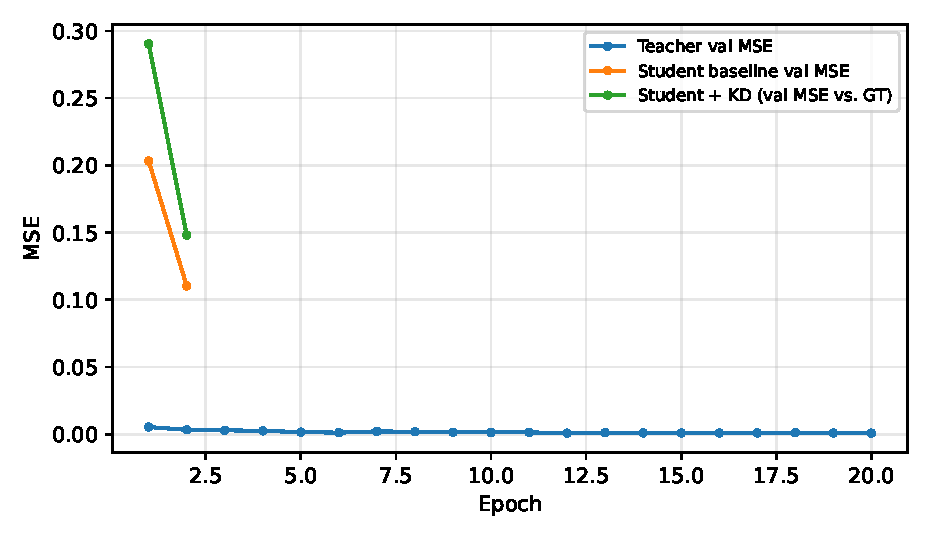
\includegraphics[width=\linewidth]{loss_curves.pdf}
  \caption{Validation MSE vs.\ epoch. For the KD run we plot the MSE between student and ground truth on the validation set to compare fairly with supervised training.}
  \label{fig:loss}
\end{figure}

\begin{figure}[H]
  \centering
  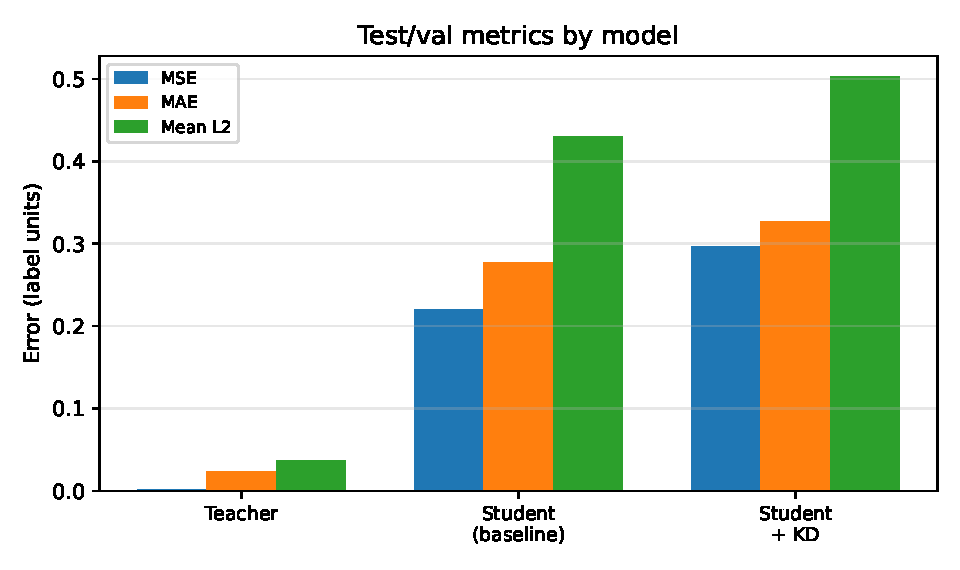
\includegraphics[width=\linewidth]{metrics_compare.pdf}
  \caption{Bar comparison of MSE, MAE, and mean Euclidean error across models.}
  \label{fig:metrics}
\end{figure}

\begin{figure}[H]
  \centering
  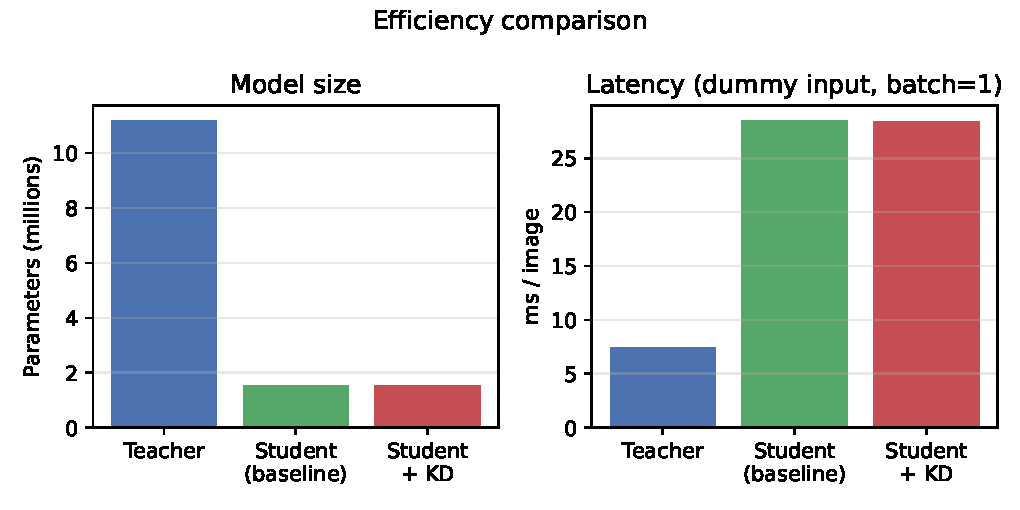
\includegraphics[width=\linewidth]{efficiency.pdf}
  \caption{Parameter count (millions) and per-image latency on a dummy input (batch size one).}
  \label{fig:eff}
\end{figure}

\subsection{Interpretation}

We expect the teacher to achieve the lowest regression error among the three models, at the cost of more parameters and higher latency. The student baseline illustrates what a compact architecture achieves with labels alone. KD typically reduces the student's error toward the teacher's behavior; gains depend on $\alpha$, optimizer settings, and whether the teacher is strong relative to the student capacity. If KD underperforms, try smaller $\alpha$, longer training, or ensuring the teacher is well converged.

\section{Discussion}

This project intentionally uses MSE in image-space gaze coordinates for clarity. Published gaze work often reports \emph{angular error} between predicted and true gaze directions in camera space; adopting that metric requires consistent 3D geometry or camera calibration and is an important next step. Stronger data augmentation (color jitter, controlled crops) may improve generalization but must respect how labels are defined. Feature-level distillation or logits-style matching could provide richer supervision than output MSE alone. For deployment, exporting the student to ONNX and optimizing with TensorRT (NVIDIA) or mobile runtimes (Core ML, TFLite) would align evaluation with production latency.

\section*{References}

\begin{thebibliography}{9}

\bibitem{zhang15mpiigaze}
X.~Zhang, Y.~Sugano, M.~Fritz, and A.~Bulling,
\newblock Appearance-based gaze estimation in the wild,
\newblock in \emph{Proc.\ IEEE CVPR}, 2015.

\bibitem{hinton15kd}
G.~Hinton, O.~Vinyals, and J.~Dean,
\newblock Distilling the knowledge in a neural network,
\newblock \emph{arXiv:1503.02531}, 2015.

\bibitem{howard19mobilenetv3}
A.~Howard, M.~Sandler, G.~Chu, et al.,
\newblock Searching for MobileNetV3,
\newblock in \emph{Proc.\ IEEE ICCV}, 2019.

\end{thebibliography}

\end{document}
